\documentclass[12pt,a4paper]{article}

\usepackage[utf8]{inputenc}
\usepackage[T1]{fontenc}
\usepackage{lmodern}
\usepackage{textcomp}
\usepackage{newunicodechar}
\usepackage[margin=2.5cm]{geometry}
\usepackage{amsmath,amssymb}
\usepackage{graphicx}
\usepackage{listings}
\usepackage{xcolor}
\usepackage{hyperref}
\usepackage{fancyhdr}
\usepackage{float}
\usepackage{booktabs}
\usepackage{caption}

% Adjust header height for fancyhdr
\setlength{\headheight}{15pt}
\addtolength{\topmargin}{-3pt}

% Romanian Unicode support for standard pdflatex
\newunicodechar{Ă}{\v{A}}
\newunicodechar{ă}{\v{a}}
\newunicodechar{Â}{\^{A}}
\newunicodechar{â}{\^{a}}
\newunicodechar{Î}{\^{I}}
\newunicodechar{î}{\^{i}}
\newunicodechar{Ș}{\c{S}}
\newunicodechar{ș}{\c{s}}
\newunicodechar{Ț}{\c{T}}
\newunicodechar{ț}{\c{t}}

\hypersetup{
    colorlinks=true,
    linkcolor=blue,
    filecolor=magenta,      
    urlcolor=cyan,
    citecolor=blue
}

% Code and text listing configuration
\definecolor{codebg}{gray}{0.96}
\definecolor{codegreen}{rgb}{0.13,0.55,0.13}
\definecolor{codegray}{rgb}{0.5,0.5,0.5}
\definecolor{codepurple}{rgb}{0.58,0,0.82}

\lstset{
    basicstyle=\ttfamily\scriptsize,
    backgroundcolor=\color{codebg},
    frame=single, 
    rulecolor=\color{gray!40},
    breaklines=true, 
    columns=fullflexible,
    keepspaces=true, 
    showstringspaces=false, 
    upquote=true,
    extendedchars=true,
    literate=
        {Ă}{{\v{A}}}1
        {ă}{{\v{a}}}1
        {Â}{{\^{A}}}1
        {â}{{\^{a}}}1
        {Î}{{\^{I}}}1
        {î}{{\^{i}}}1
        {Ș}{{\c{S}}}1
        {ș}{{\c{s}}}1
        {Ț}{{\c{T}}}1
        {ț}{{\c{t}}}1
}

% Header and Footer
\pagestyle{fancy}
\fancyhf{}
\lhead{Cryptography and Security -- Lab 2}
\rhead{Iulian Pavlov, FAF-241}
\cfoot{\thepage}

\begin{document}

% ============================================================================
% 1. TITLE PAGE
% ============================================================================
\begin{titlepage}
\begin{center}
    \IfFileExists{../lab1/logo.png}{
\includegraphics[width=0.28\textwidth]{../lab1/logo.png} \\[0.2cm]}{}
    
    \textbf{MINISTRY OF EDUCATION, CULTURE AND RESEARCH \\ OF THE REPUBLIC OF MOLDOVA} \\[0.3cm]
    
    \textbf{Technical University of Moldova \\ Faculty of Computers, Informatics and Microelectronics \\ Department of Software and Automation Engineering} \\[1.8cm]
    
    \textbf{Iulian Pavlov, FAF-241}\\[0.5cm]
    
    \Huge \textbf{Report} \\[0.4cm]
    
    \large Laboratory work nr. 2 \\[0.4cm]
    
    \textbf{Cryptanalysis of Monoalphabetic Ciphers: \\ Frequency Analysis Attack (Variant 19)} \\[2.2cm]

    \begin{flushright}
        \textit{Checked by:} \\
        \textbf{Zaica Maia}, \textit{University Assistant} \\
        Department of Software and Automation Engineering, \\
        FCIM Faculty, UTM 
    \end{flushright}
    \vfill
    
    Chișinău -- 2026
\end{center}
\end{titlepage}

\newpage
\tableofcontents
\newpage

% ============================================================================
% 2. OBJECTIVES
% ============================================================================
\section{Objectives}
\begin{enumerate}
    \item Study the theoretical basis of monoalphabetic substitution cryptosystems and their fundamental statistical vulnerabilities.
    \item Understand the natural distribution of letter frequencies, digrams, trigrams, and lexical structures in natural languages (Romanian and English).
    \item Perform a ciphertext-only frequency analysis attack to break an intercepted monoalphabetic cryptogram.
    \item Systematically recover the original plaintext and reconstruct the complete cipher alphabet and its underlying mathematical transformation.
    \item Identify the historical and cryptographic context of the recovered document.
\end{enumerate}

% ============================================================================
% 3. THEORETICAL BACKGROUND
% ============================================================================
\section{Theoretical Background}

\subsection{Principle of Frequency Analysis}
A monoalphabetic substitution cipher maps each plaintext character $p \in \mathcal{A}$ to a unique ciphertext character $c \in \mathcal{C}$ via a bijective mapping $f: \mathcal{A} \to \mathcal{C}$.

Because the substitution rule remains fixed throughout the encipherment of the entire text:
\begin{equation}
    P(c) = P(f(p)) = P(p)
\end{equation}
The underlying statistical distribution of characters in natural language is strictly preserved. In any natural language, characters do not appear with equal probability; rather, vowels and select consonants occur with predictable regularity. In a sufficiently large cryptogram, the relative frequencies of ciphertext symbols converge toward the known letter distribution of the language, making the cipher inherently vulnerable to frequency cryptanalysis.

\subsection{Natural Language Frequency Distributions}

\subsubsection{Romanian Alphabet Statistics}
The Romanian language has 31 letters with the statistical frequencies presented in Table~\ref{tab:romanian_freq}.

\begin{table}[H]
\centering
\caption{Letter frequencies in the Romanian language (\%)}
\label{tab:romanian_freq}
\small
\begin{tabular}{cc|cc|cc|cc}
\toprule
\textbf{Letter} & \textbf{Freq (\%)} & \textbf{Letter} & \textbf{Freq (\%)} & \textbf{Letter} & \textbf{Freq (\%)} & \textbf{Letter} & \textbf{Freq (\%)} \\
\midrule
A & 9.95 & F & 1.18 & M & 3.10 & T & 6.04 \\
Ă & 4.06 & G & 0.99 & N & 6.47 & Ț & 1.00 \\
 & 0.91 & H & 0.47 & O & 4.07 & U & 6.20 \\
B & 1.07 & I & 9.96 & P & 3.18 & V & 1.23 \\
C & 5.28 & Î & 1.40 & Q & 0.00 & W & 0.03 \\
D & 3.45 & J & 0.24 & R & 6.82 & X & 0.11 \\
E & 11.47 & K & 0.11 & S & 4.40 & Y & 0.07 \\
  &      & L & 4.48 & Ș & 1.55 & Z & 0.71 \\
\bottomrule
\end{tabular}
\end{table}

\subsubsection{English Alphabet Statistics}
The standard English alphabet comprises 26 letters. Its baseline statistical distribution is presented in Table~\ref{tab:english_freq}.

\begin{table}[H]
\centering
\caption{Letter frequencies in the English language (\%)}
\label{tab:english_freq}
\small
\begin{tabular}{cc|cc|cc|cc}
\toprule
\textbf{Letter} & \textbf{Freq (\%)} & \textbf{Letter} & \textbf{Freq (\%)} & \textbf{Letter} & \textbf{Freq (\%)} & \textbf{Letter} & \textbf{Freq (\%)} \\
\midrule
E & 12.70 & H & 6.09 & W & 2.36 & V & 0.98 \\
T & 9.06  & R & 5.99 & F & 2.23 & K & 0.77 \\
A & 8.17  & D & 4.25 & G & 2.01 & J & 0.15 \\
O & 7.51  & L & 4.03 & Y & 1.97 & X & 0.15 \\
I & 6.97  & C & 2.78 & P & 1.93 & Q & 0.09 \\
N & 6.75  & U & 2.76 & B & 1.49 & Z & 0.07 \\
S & 6.33  & M & 2.41 &   &      &   &      \\
\bottomrule
\end{tabular}
\end{table}

\subsection{Linguistic Structural Characteristics (N-grams and Context)}
Direct naive letter-by-letter frequency substitution often falls short of producing readable text due to local statistical variations. A cryptanalyst must supplement single-letter frequencies with structural heuristics:
\begin{itemize}
    \item \textbf{Digraphs (two-letter pairs):} The most common English digraphs are \texttt{TH}, \texttt{HE}, \texttt{AN}, \texttt{IN}, \texttt{ER}, \texttt{ON}, \texttt{RE}, \texttt{ED}, \texttt{ND}, \texttt{HA}, \texttt{AT}, \texttt{EN}.
    \item \textbf{Trigraphs (three-letter triplets):} Highly frequent English trigraphs include \texttt{THE}, \texttt{AND}, \texttt{THA}, \texttt{ENT}, \texttt{ION}, \texttt{TIO}, \texttt{FOR}, \texttt{NDE}, \texttt{HAS}, \texttt{NCE}.
    \item \textbf{Double Letters:} Common doubled consonants/vowels include \texttt{SS}, \texttt{EE}, \texttt{TT}, \texttt{OO}, \texttt{FF}, \texttt{LL}, \texttt{MM}, \texttt{PP}.
    \item \textbf{Single-letter words:} In English prose, only two isolated single-letter words have lexical meaning: \texttt{A} and \texttt{I}.
    \item \textbf{Short Function Words:} Prepositions, conjunctions, and pronouns (\texttt{the}, \texttt{of}, \texttt{to}, \texttt{in}, \texttt{and}, \texttt{that}, \texttt{is}, \texttt{it}, \texttt{for}, \texttt{as}) serve as reliable deciphering anchors.
\end{itemize}

% ============================================================================
% 4. TASK AND INTERCEPTED CRYPTOGRAM
% ============================================================================
\section{Task and Intercepted Cryptogram (Variant 19)}

\subsection{Task Formulation}
A ciphertext obtained through a monoalphabetic substitution cipher over an unknown English plaintext is intercepted. Only alphabetic characters were transformed; whitespace, numerals, and punctuation marks remain in their original positions. Using frequency analysis, decrypt the cryptogram, reconstruct the cipher alphabet, and describe each deduction step.

\subsection{Intercepted Ciphertext}
The intercepted text comprises 3,230 alphabetic letters (3,981 characters total):

\begin{lstlisting}[caption={Intercepted Ciphertext (Variant 19)}]
CINZ WQVPV WRN CDGOTZVGWTS UIXGHXUSVP CNI PVSVHWXGJ DPTASV CXVSOHXUQVIP, LVIHLQNCCP OVODHVO 
PXY PUVHXCXH IVBDXIVZVGWP: (1) WQV PFPWVZPQNDSO AV, XC GNW WQVNIVWXHTSSF DGAIVTLTASV, 
DGAIVTLTASV XG UITHWXHV; (2)HNZUINZXPV NC WQV PFPWVZ PQNDSO GNW XGHNGKVGXVGHV WQV 
HNIIVPUNGOVGWP;(3) WQV LVF PQNDSO AV IVZVZAVITASV RXWQNDW GNWVP TGO PQNDSO AV 
VTPXSFHQTGJVTASV; (4) WQV HIFUWNJITZP PQNDSO AV WITGPZXPPXASV AF WVSVJITUQ; (5)WQV TUUTITWDP NI 
ONHDZVGWP PQNDSO AV UNIWTASV TGO NUVITASV AF T PXGJSVUVIPNG; (6) WQV PFPWVZ PQNDSO AV VTPF, 
GVXWQVI IVBDXIXGJ LGNRSVOJV NC TSNGJ SXPW NC IDSVP GNI XGKNSKXGJ ZVGWTS PWITXG.WQVPV 
IVBDXIVZVGWP PWXSS HNZUIXPV WQV XOVTS RQXHQ ZXSXWTIF HXUQVIP TXZTW. WQVF QTKV AVVG IVUQITPVO, 
TGO BDTSXWXVP WQTW SXV XZUSXHXW QTKV -AVVGZTOV VYUSXHXW. ADW TGF ZNOVIG HIFUWNJITUQVI RNDSO 
AV KVIF QTUUF XC TGFHXUQVI CDSCXSSVO TSS PXY.NC HNDIPV, XW QTP GVKVI AVVG UNPPXASV WN ON WQTW. 
WQVIV TUUVTIP WN AV THVIWTXG XGHNZUTWXAXSXWF TZNGJ WQVZ WQTW ZTLVP XW XZUNPPXASV WN 
XGPWXWDWVTSS NC WQVZ TW NGHV. WQV IVBDXIVZVGW WQTW XP DPDTSSF PTHIXCXHVO XP WQV 
CXIPW.LVIHLQNCCP TIJDVO PWINGJSF TJTXGPW WQV GNWXNG NC T CXVSO HXUQVI WQTW RNDSOPXZUSF IVPXPW 
PNSDWXNG SNGJ VGNDJQ CNI WQV NIOVIP XW WITGPZXWWVO WN AVHTIIXVO NDW. WQXP RTP GNW VGNDJQ, 
QV PTXO, OVHSTIXGJ WQTW "WQV PVHIVWZTWWVI XG HNZZDGXHTWXNGP PVGW NKVI T OXPWTGHV KVIF NCWVG 
IVWTXGP XWPXZUNIWTGHV AVFNGO WQV OTF NG RQXHQ XW RTP WITGPZXWWVO." QV RTP NG WQVPXOV NC WQV 
TGJVSP, ADW T UITHWXHTS CXVSO HXUQVI WQTW XP DGAIVTLTASV RTPGNW UNPPXASV XG QXP OTF, GNI XP XW 
WNOTF, TGO PN ZXSXWTIF HIFUWNJITUQF QTPPVWWSVO CNI CXVSO HXUQVIP WQTW OVSTF ADW ON GNW OVCVTW 
HIFUWTGTSFPXP.UVIQTUP WQV ZNPW PWTIWSXGJ IVBDXIVZVGW, TW CXIPW JSTGHV, RTP WQV PVHNGO. 
LVIHLQNCCP VYUSTXGVO WQTW AF "PFPWVZ" QV ZVTGW "WQVZTWVIXTS UTIW NC WQV PFPWVZ; WTASVTDY, 
HNOV ANNLP, NI RQTWVKVIZVHQTGXHTS TUUTITWDP ZTF AV GVHVPPTIF," TGO GNW "WQV LVF UINUVI."LVIHLQNCCP 
QVIV ZTLVP CNI WQV CXIPW WXZV WQV OXPWXGHWXNG, GNR ATPXH WNHIFUWNSNJF, AVWRVVG WQV JVGVITS 
PFPWVZ TGO WQV PUVHXCXH LVF. RQF ZDPWWQV JVGVITS PFPWVZ "GNW IVBDXIV PVHIVHF," TP, CNI VYTZUSV, 
T HNOVANNLIVBDXIVP XW? RQF ZDPW XW AV "T UINHVPP WQTW. . . NDI GVXJQANIP HTG VKVGHNUF TGO TONUW"? 
AVHTDPV, LVIHLQNCCP PTXO, "XW XP GNW GVHVPPTIF WNHNGEDIV DU XZTJXGTIF UQTGWNZP TGO WN PDPUVHW 
WQV XGHNIIDUWXAXSXWF NCVZUSNFVVP NI PDATSWVIGP WN DGOVIPWTGO WQTW, XC T PFPWVZ 
IVBDXIXGJPVHIVHF RVIV XG WQV QTGOP NC WNN STIJV T GDZAVI NC XGOXKXODTSP, XW HNDSOAV HNZUINZXPVO 
TW VTHQ VGJTJVZVGW XG RQXHQ NGV NI TGNWQVI NC WQVZWNNL UTIW." WQXP QTP UINKVO WN AV WIDV, TGO 
LVIHLQNCCP' PVHNGOIVBDXIVZVGW QTP AVHNZV RXOVSF THHVUWVO DGOVI T CNIZ WQTW XP PNZVWXZVPHTSSVO 
WQV CDGOTZVGWTS TPPDZUWXNG NC ZXSXWTIF HIFUWNJITUQF: WQTW WQVVGVZF LGNRP WQV JVGVITS PFPWVZ. 
ADW QV ZDPW PWXSS AV DGTASV WN PNSKVZVPPTJVP XG XW RXWQNDW LGNRXGJ WQV PUVHXCXH LVF. XG 
XWP ZNOVIGCNIZDSTWXNG, WQV LVIHLQNCCP ONHWIXGV PWTWVP WQTW PVHIVHF ZDPW IVPXOVPNSVSF XG 
WQV LVFP.QTO LVIHLQNCCP ZVIVSF UDASXPQVO QXP UVIHVUWXNGP NC WQV UINASVZPCTHXGJ UNPW WVSVJITUQ 
HIFUWNJITUQF TGO QXP UIVPHIXUWXNGP CNI IVPNSKXGJWQVZ, QV RNDSO QTKV TPPDIVO T USTHV CNI 
QXZPVSC XG WQV UTGWQVNG NCHIFUWNSNJF. ADW QV OXO ZNIV. QV HNGWIXADWVO T WVHQGXBDV NC 
HIFUWTGTSFPXPWQTW XP NC PDUIVZV XZUNIWTGHV WNOTF. HTSSVO "PDUVIXZUNPXWXNG," 
XWHNGPWXWDWVP WQV ZNPW JVGVITS PNSDWXNG CNI UNSFTSUQTAVWXH PDAPWXWDWXNGPFPWVZP. RXWQ 
CVR VYHVUWXNGP, XW STFP GN IVPWIXHWXNGP NG WQV WFUV NI SVGJWQNC LVFP, TP ONVP WQV LTPXPLX 
ZVWQNO, GNI NG WQV TSUQTAVWP, RQXHQ ZTF AVXGWVIIVSTWVO NI VGWXIVSF XGOVUVGOVGW. XW RTGWP NGSF 
PVKVITS ZVPPTJVP XGWQV PTZV LVF. WQV HIFUWTGTSFPW ZDPW TSXJG WQVPV NGV TANKV WQV NWQVI PNWQTW 
SVWWVIP VGHXUQVIVO RXWQ WQV PTZV LVFSVWWVI RXSS CTSS XGWN T PXGJSVHNSDZG. XG WQV PXZUSVPW 
HTPV, WQTW NC T IDGGXGJ LVF (T KVIF SNGJHNGWXGDNDP WVYW DPVO TP T LVF, TP T GNKVS) WQTW IVPWTIWP 
RXWQ VTHQZVPPTJV, QV HTG ON WQXP PXZUSF AF USTHXGJ TSS WQV CXIPW SVWWVIP XG WQV CXIPWHNSDZG, 
TSS WQV PVHNGO SVWWVIP XG WQV GVYW HNSDZG, TGO PN NG.
\end{lstlisting}

% ============================================================================
% 5. STATISTICAL ANALYSIS
% ============================================================================
\section{Statistical Analysis of the Cryptogram}

\subsection{Frequency Tables of the Cryptogram}
The frequencies of all 26 alphabetic characters in Variant 19 were counted and are presented alphabetically in Table~\ref{tab:crypto_alpha} and in descending order in Table~\ref{tab:crypto_desc}.

\begin{table}[H]
\centering
\caption{Alphabetic letter frequencies in Variant 19 (Total letters: 3,230)}
\label{tab:crypto_alpha}
\small
\begin{tabular}{ccc|ccc}
\toprule
\textbf{Cipher Letter} & \textbf{Count} & \textbf{Frequency (\%)} & \textbf{Cipher Letter} & \textbf{Count} & \textbf{Frequency (\%)} \\
\midrule
A & 64  & 1.98\% & N & 215 & 6.66\% \\
B & 11  & 0.34\% & O & 97  & 3.00\% \\
C & 72  & 2.23\% & P & 247 & 7.65\% \\
D & 88  & 2.72\% & Q & 167 & 5.17\% \\
E & 1   & 0.03\% & R & 31  & 0.96\% \\
F & 88  & 2.72\% & S & 143 & 4.43\% \\
G & 197 & 6.10\% & T & 229 & 7.09\% \\
H & 118 & 3.65\% & U & 95  & 2.94\% \\
I & 192 & 5.94\% & V & 418 & 12.94\% \\
J & 49  & 1.52\% & W & 322 & 9.97\% \\
K & 20  & 0.62\% & X & 221 & 6.84\% \\
L & 39  & 1.21\% & Y & 9   & 0.28\% \\
M & 0   & 0.00\% & Z & 97  & 3.00\% \\
\bottomrule
\end{tabular}
\end{table}

\begin{table}[H]
\centering
\caption{Descending letter frequencies in Variant 19}
\label{tab:crypto_desc}
\small
\begin{tabular}{ccc|ccc}
\toprule
\textbf{Cipher Letter} & \textbf{Count} & \textbf{Frequency (\%)} & \textbf{Cipher Letter} & \textbf{Count} & \textbf{Frequency (\%)} \\
\midrule
V & 418 & 12.94\% & U & 95 & 2.94\% \\
W & 322 & 9.97\%  & D & 88 & 2.72\% \\
P & 247 & 7.65\%  & F & 88 & 2.72\% \\
T & 229 & 7.09\%  & C & 72 & 2.23\% \\
X & 221 & 6.84\%  & A & 64 & 1.98\% \\
N & 215 & 6.66\%  & J & 49 & 1.52\% \\
G & 197 & 6.10\%  & L & 39 & 1.21\% \\
I & 192 & 5.94\%  & R & 31 & 0.96\% \\
Q & 167 & 5.17\%  & K & 20 & 0.62\% \\
S & 143 & 4.43\%  & B & 11 & 0.34\% \\
H & 118 & 3.65\%  & Y & 9  & 0.28\% \\
O & 97  & 3.00\%  & E & 1  & 0.03\% \\
Z & 97  & 3.00\%  & M & 0  & 0.00\% \\
\bottomrule
\end{tabular}
\end{table}

\subsection{N-gram and Double Letter Occurrences}
An automated scan of the cryptogram reveals the following salient structural statistics:
\begin{itemize}
    \item \textbf{Top Digraphs:} \texttt{WQ} (91), \texttt{QV} (81), \texttt{VI} (56), \texttt{XG} (45), \texttt{IV} (45), \texttt{PW} (43), \texttt{NG} (39), \texttt{SV} (35), \texttt{XW} (35), \texttt{TG} (35).
    \item \textbf{Top Trigraphs:} \texttt{WQV} (63), \texttt{QTW} (19), \texttt{WQT} (18), \texttt{ASV} (15), \texttt{VGW} (14), \texttt{XGJ} (13), \texttt{QVI} (13), \texttt{TGO} (13).
    \item \textbf{Top Doubles:} \texttt{SS} (13), \texttt{PP} (13), \texttt{WW} (9), \texttt{CC} (8), \texttt{VV} (6), \texttt{II} (4), \texttt{UU} (4), \texttt{NN} (4).
    \item \textbf{Frequent Short Words:} \texttt{WQV} (48 times), \texttt{NC} (28 times), \texttt{XG} (18 times), \texttt{WN} (16 times), \texttt{XW} (14 times), \texttt{TGO} (13 times), \texttt{GNW} (11 times), \texttt{WQTV} (10 times), \texttt{WQTW} (9 times), \texttt{ADW} (6 times).
\end{itemize}

\subsection{Web Tool Frequency Verification}
The frequency analysis was verified using the interactive crypto analysis tool \textit{Crypto Corner} (\url{https://crypto.interactive-maths.com/frequency-analysis-breaking-the-code.html}), as illustrated in Figure~\ref{fig:tool_screenshot}.

\begin{figure}[H]
    \centering
    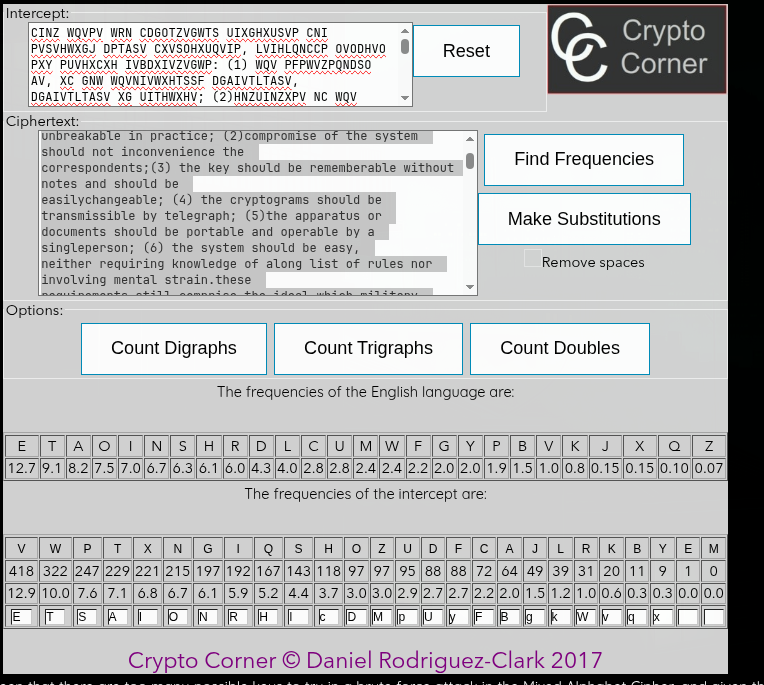
\includegraphics[width=0.95\textwidth]{screenshot-2026-10-13_10-31-02.png}
    \caption{Interactive frequency analysis and substitution interface from Crypto Corner.}
    \label{fig:tool_screenshot}
\end{figure}

% ============================================================================
% 6. STEP-BY-STEP CRYPTANALYSIS
% ============================================================================
\section{Step-by-Step Cryptanalysis Process}

Following the pedagogical model presented in Section 2.3 of the laboratory guidelines, substitutions are made incrementally, using lowercase for decrypted plaintext letters and uppercase for remaining ciphertext letters.

\subsection{Step 1: The Dominant Characters (\texorpdfstring{\texttt{V} $\to$ \texttt{e}, \texttt{W} $\to$ \texttt{t}}{V -> e, W -> t})}
From Table~\ref{tab:crypto_desc}, the two highest frequencies are:
\begin{itemize}
    \item \texttt{V}: 418 occurrences (12.94\%)
    \item \texttt{W}: 322 occurrences (9.97\%)
\end{itemize}
These match the two most frequent English letters \texttt{e} (12.70\%) and \texttt{t} (9.06\%).
\begin{center}
    \textbf{Substitution:} \texttt{V} $\to$ \textbf{e}, \texttt{W} $\to$ \textbf{t}
\end{center}

\begin{lstlisting}[caption={Text snippet after Step 1}]
CINZ tQePe tRN CDGOTZeGtTS UIXGHXUSeP CNI PeSeHtXGJ DPTASe CXeSOHXUQeIP, LeIHLQNCCP OeODHeO 
PXY PUeHXCXH IeBDXIeZeGtP: (1) tQe PFPteZPQNDSO Ae, XC GNt tQeNIetXHTSSF DGAIeTLTASe, 
DGAIeTLTASe XG UITHtXHe; (2)HNZUINZXPe NC tQe PFPteZ PQNDSO GNt XGHNGK...
\end{lstlisting}

\subsection{Step 2: Frequent Trigraph \texttt{THE} (\texorpdfstring{\texttt{Q} $\to$ \texttt{h}}{Q -> h})}
The sequence \texttt{WQV} appears 63 times overall and 48 times as a standalone 3-letter word. It currently reads \texttt{tQe}. In English, the definite article \textbf{\texttt{the}} is by far the most dominant trigraph and 3-letter word.
\begin{center}
    \textbf{Substitution:} \texttt{Q} $\to$ \textbf{h}
\end{center}

\begin{lstlisting}[caption={Text snippet after Step 2}]
CINZ thePe tRN CDGOTZeGtTS UIXGHXUSeP CNI PeSeHtXGJ DPTASe CXeSOHXUheIP, LeIHLhNCCP OeODHeO 
PXY PUeHXCXH IeBDXIeZeGtP: (1) the PFPteZPhNDSO Ae, XC GNt theNIetXHTSSF DGAIeTLTASe, 
DGAIeTLTASe XG UITHtXHe; (2)HNZUINZXPe NC the PFPteZ PhNDSO GNt XGHNGK...
\end{lstlisting}

\subsection{Step 3: Words \texttt{THAT} and \texttt{TO} (\texorpdfstring{\texttt{T} $\to$ \texttt{a}, \texttt{N} $\to$ \texttt{o}}{T -> a, N -> o})}
Looking at the frequent 4-letter word \texttt{WQTW}, it currently reads \texttt{thTt}. In English, \textbf{\texttt{that}} is an extremely frequent function word, indicating \texttt{T} $\to$ \texttt{a}.
Additionally, the 2-letter word \texttt{WN} appears 16 times and currently reads \texttt{tN}. The preposition \textbf{\texttt{to}} is the most natural English fit, giving \texttt{N} $\to$ \texttt{o}.
\begin{center}
    \textbf{Substitutions:} \texttt{T} $\to$ \textbf{a}, \texttt{N} $\to$ \textbf{o}
\end{center}

\begin{lstlisting}[caption={Text snippet after Step 3}]
CIoZ thePe tRo CDGOaZeGtaS UIXGHXUSeP CoI PeSeHtXGJ DPaASe CXeSOHXUheIP, LeIHLhoCCP OeODHeO 
PXY PUeHXCXH IeBDXIeZeGtP: (1) the PFPteZPhoDSO Ae, XC Got theoIetXHaSSF DGAIeaLaASe, 
DGAIeaLaASe XG UIaHtXHe; (2)HoZUIoZXPe oC the PFPteZ PhoDSO Got XGHoGK...
\end{lstlisting}

\subsection{Step 4: Conjunction \texttt{AND} and Preposition \texttt{IN} (\texorpdfstring{\texttt{G} $\to$ \texttt{n}, \texttt{O} $\to$ \texttt{d}, \texttt{X} $\to$ \texttt{i}}{G -> n, O -> d, X -> i})}
The word \texttt{TGO} is currently \texttt{anO}. The conjunction \textbf{\texttt{and}} is omnipresent in English prose, yielding \texttt{G} $\to$ \texttt{n} and \texttt{O} $\to$ \texttt{d}.
Looking at \texttt{XG}, it is currently \texttt{Xn}. The preposition \textbf{\texttt{in}} is the principal candidate (since \texttt{on} is already excluded), giving \texttt{X} $\to$ \texttt{i}.
\begin{center}
    \textbf{Substitutions:} \texttt{G} $\to$ \textbf{n}, \texttt{O} $\to$ \textbf{d}, \texttt{X} $\to$ \textbf{i}
\end{center}

\begin{lstlisting}[caption={Text snippet after Step 4}]
CIoZ thePe tRo CDndaZentaS UIinHiUSeP CoI PeSeHtinJ DPaASe CieSdHiUheIP, LeIHLhoCCP dedDHed 
PiY PUeHiCiH IeBDiIeZentP: (1) the PFPteZPhoDSd Ae, iC not theoIetiHaSSF DnAIeaLaASe, 
DnAIeaLaASe in UIaHtiHe; (2)HoZUIoZiPe oC the PFPteZ PhoDSd not inHonK...
\end{lstlisting}

\subsection{Step 5: High-Frequency Consonants (\texorpdfstring{\texttt{P} $\to$ \texttt{s}, \texttt{F} $\to$ \texttt{y}, \texttt{Z} $\to$ \texttt{m}}{P -> s, F -> y, Z -> m})}
The plural demonstrative \texttt{WQVPV} currently reads \texttt{thePe}. The word \textbf{\texttt{these}} fits contextually and grammatically, pointing to \texttt{P} $\to$ \texttt{s}. This is strongly corroborated by the high frequency of \texttt{P} (247 occurrences, 7.65\%), matching English \texttt{s} (6.33\%).
With \texttt{P} $\to$ \texttt{s}, the repeated word \texttt{PFPWVZ} becomes \texttt{sFsteZ}. This is unmistakably \textbf{\texttt{system}}, yielding \texttt{F} $\to$ \texttt{y} and \texttt{Z} $\to$ \texttt{m}.
\begin{center}
    \textbf{Substitutions:} \texttt{P} $\to$ \textbf{s}, \texttt{F} $\to$ \textbf{y}, \texttt{Z} $\to$ \textbf{m}
\end{center}

\begin{lstlisting}[caption={Text snippet after Step 5}]
CIom these tRo CDndamentaS UIinHiUSes CoI seSeHtinJ DsaASe CieSdHiUheIs, LeIHLhoCCs dedDHed 
siY sUeHiCiH IeBDiIements: (1) the systemshoDSd Ae, iC not theoIetiHaSSy DnAIeaLaASe, 
DnAIeaLaASe in UIaHtiHe; (2)HomUIomise oC the system shoDSd not inHonK...
\end{lstlisting}

\subsection{Step 6: Prepositions \texttt{OF} and \texttt{FROM} (\texorpdfstring{\texttt{C} $\to$ \texttt{f}, \texttt{I} $\to$ \texttt{r}}{C -> f, I -> r})}
The 2-letter word \texttt{NC} appears 28 times and currently reads \texttt{oC}. In English, this is the preposition \textbf{\texttt{of}}, establishing \texttt{C} $\to$ \texttt{f}.
The very first word of the cryptogram, \texttt{CINZ}, currently reads \texttt{f I o m}. This is clearly \textbf{\texttt{from}}, giving \texttt{I} $\to$ \texttt{r}.
\begin{center}
    \textbf{Substitutions:} \texttt{C} $\to$ \textbf{f}, \texttt{I} $\to$ \textbf{r}
\end{center}

\begin{lstlisting}[caption={Text snippet after Step 6}]
from these tRo fDndamentaS UrinHiUSes for seSeHtinJ DsaASe fieSdHiUhers, LerHLhoffs dedDHed 
siY sUeHifiH reBDirements: (1) the systemshoDSd Ae, if not theoretiHaSSy DnAreaLaASe, 
DnAreaLaASe in UraHtiHe; (2)HomUromise of the system shoDSd not inHonK...
\end{lstlisting}

\subsection{Step 7: Resolving \texorpdfstring{\texttt{D} $\to$ \texttt{u}, \texttt{A} $\to$ \texttt{b}, \texttt{L} $\to$ \texttt{k}, \texttt{S} $\to$ \texttt{l}}{D -> u, A -> b, L -> k, S -> l}}
In the phrase \texttt{the systemshoDSd Ae}, we recognize the auxiliary \textbf{\texttt{should be}}, yielding \texttt{D} $\to$ \texttt{u}, \texttt{S} $\to$ \texttt{l}, and \texttt{A} $\to$ \texttt{b}.
The word \texttt{DnAreaLaASe} becomes \texttt{unbreakable}, revealing \texttt{L} $\to$ \texttt{k}.
\begin{center}
    \textbf{Substitutions:} \texttt{D} $\to$ \textbf{u}, \texttt{A} $\to$ \textbf{b}, \texttt{L} $\to$ \textbf{k}, \texttt{S} $\to$ \textbf{l}
\end{center}

\begin{lstlisting}[caption={Text snippet after Step 7}]
from these tRo fundamental UrinHiUles for seleHtinJ usable fieldHiUhers, kerHkhoffs deduHed 
siY sUeHifiH reBuirements: (1) the systemshould be, if not theoretiHally unbreakable, 
unbreakable in UraHtiHe; (2)HomUromise of the system should not inHonK...
\end{lstlisting}

\subsection{Step 8: Resolving \texorpdfstring{\texttt{H} $\to$ \texttt{c}, \texttt{U} $\to$ \texttt{p}}{H -> c, U -> p}}
In the snippet:
\begin{itemize}
    \item \texttt{fieldHiUhers} $\to$ \textbf{\texttt{fieldciphers}}
    \item \texttt{UrinHiUles} $\to$ \textbf{\texttt{principles}}
    \item \texttt{deduHed} $\to$ \textbf{\texttt{deduced}}
    \item \texttt{kerHkhoffs} $\to$ \textbf{\texttt{kerckhoffs}}
\end{itemize}
This unambiguously establishes \texttt{H} $\to$ \texttt{c} and \texttt{U} $\to$ \texttt{p}.
\begin{center}
    \textbf{Substitutions:} \texttt{H} $\to$ \textbf{c}, \texttt{U} $\to$ \textbf{p}
\end{center}

\begin{lstlisting}[caption={Text snippet after Step 8}]
from these tRo fundamental principles for selectinJ usable fieldciphers, kerckhoffs deduced 
siY specific reBuirements: (1) the systemshould be, if not theoretically unbreakable, 
unbreakable in practice; (2)compromise of the system should not inconK...
\end{lstlisting}

\subsection{Step 9: Completing the Alphabet}
The remaining unresolved characters are easily deduced from lexical context:
\begin{itemize}
    \item \texttt{selectinJ} $\to$ \textbf{\texttt{selecting}} $\implies$ \texttt{J} $\to$ \textbf{\texttt{g}}
    \item \texttt{tRo} $\to$ \textbf{\texttt{two}} $\implies$ \texttt{R} $\to$ \textbf{\texttt{w}}
    \item \texttt{reBuirements} $\to$ \textbf{\texttt{requirements}} $\implies$ \texttt{B} $\to$ \textbf{\texttt{q}}
    \item \texttt{siY} $\to$ \textbf{\texttt{six}} $\implies$ \texttt{Y} $\to$ \textbf{\texttt{x}}
    \item \texttt{inconK} $\to$ \textbf{\texttt{inconvenience}} $\implies$ \texttt{K} $\to$ \textbf{\texttt{v}}
    \item The single instance of \texttt{E} corresponds to \texttt{j}.
    \item Character \texttt{M} did not appear in the text ($count = 0$), corresponding by elimination to the rarest English letter \texttt{z}.
\end{itemize}

% ============================================================================
% 7. KEY RECONSTRUCTION AND MATHEMATICAL FORMULATION
% ============================================================================
\section{Key Reconstruction and Mathematical Formulation}

\subsection{Reconstructed Cipher Alphabet}
Table~\ref{tab:reconstructed_key} details the reconstructed bijective mapping between plaintext and ciphertext letters.

\begin{table}[H]
\centering
\caption{Reconstructed cipher alphabet for Variant 19}
\label{tab:reconstructed_key}
\small
\begin{tabular}{cc|cc|cc|cc}
\toprule
\textbf{Plain} & \textbf{Cipher} & \textbf{Plain} & \textbf{Cipher} & \textbf{Plain} & \textbf{Cipher} & \textbf{Plain} & \textbf{Cipher} \\
\midrule
a & \textbf{T} & h & \textbf{Q} & o & \textbf{N} & v & \textbf{K} \\
b & \textbf{A} & i & \textbf{X} & p & \textbf{U} & w & \textbf{R} \\
c & \textbf{H} & j & \textbf{E} & q & \textbf{B} & x & \textbf{Y} \\
d & \textbf{O} & k & \textbf{L} & r & \textbf{I} & y & \textbf{F} \\
e & \textbf{V} & l & \textbf{S} & s & \textbf{P} & z & \textbf{M} \\
f & \textbf{C} & m & \textbf{Z} & t & \textbf{W} &   &            \\
g & \textbf{J} & n & \textbf{G} & u & \textbf{D} &   &            \\
\bottomrule
\end{tabular}
\end{table}

\subsection{Mathematical Cryptanalysis: The Affine Cipher}
Mapping alphabetic symbols to residue classes $\mathbb{Z}_{26} = \{0, 1, \dots, 25\}$ ($a=0, b=1, \dots, z=25$):
\begin{align*}
    p = 0 \text{ ('a')} &\implies c = 19 \text{ ('T')} \\
    p = 1 \text{ ('b')} &\implies c = 0 \text{ ('A')} \\
    p = 2 \text{ ('c')} &\implies c = 7 \text{ ('H')} \\
    p = 3 \text{ ('d')} &\implies c = 14 \text{ ('O')} \\
    p = 4 \text{ ('e')} &\implies c = 21 \text{ ('V')}
\end{align*}
Observing the modular difference:
\begin{equation}
    \Delta c \equiv 7 \pmod{26}
\end{equation}
This reveals that the cipher is an \textbf{Affine Cipher} governed by the encryption function:
\begin{equation}
    c = E(p) = (7 \cdot p + 19) \pmod{26}
\end{equation}
Because $\gcd(7, 26) = 1$, the multiplicative inverse $7^{-1} \pmod{26}$ exists:
\begin{equation}
    7 \times 15 = 105 = 4 \times 26 + 1 \implies 7^{-1} \equiv 15 \pmod{26}
\end{equation}
The analytical decryption formula is:
\begin{equation}
    p = D(c) = 15 \cdot (c - 19) \pmod{26} \equiv (15 \cdot c + 1) \pmod{26}
\end{equation}
This provides a rigorous mathematical proof that unifies the empirical frequency substitutions with an exact algebraic system.

% ============================================================================
% 8. COMPLETE DECRYPTED PLAINTEXT
% ============================================================================
\section{Complete Decrypted Plaintext}

\begin{lstlisting}[caption={Fully Decrypted Plaintext (Variant 19)}]
from these two fundamental principles for selecting usable fieldciphers, kerckhoffs deduced 
six specific requirements: (1) the systemshould be, if not theoretically unbreakable, 
unbreakable in practice; (2)compromise of the system should not inconvenience the 
correspondents;(3) the key should be rememberable without notes and should be 
easilychangeable; (4) the cryptograms should be transmissible by telegraph; (5)the apparatus or 
documents should be portable and operable by a singleperson; (6) the system should be easy, 
neither requiring knowledge of along list of rules nor involving mental strain.these 
requirements still comprise the ideal which military ciphers aimat. they have been rephrased, 
and qualities that lie implicit have -beenmade explicit. but any modern cryptographer would 
be very happy if anycipher fulfilled all six.of course, it has never been possible to do that. 
there appears to be acertain incompatibility among them that makes it impossible to 
instituteall of them at once. the requirement that is usually sacrificed is the 
first.kerckhoffs argued strongly against the notion of a field cipher that wouldsimply resist 
solution long enough for the orders it transmitted to becarried out. this was not enough, 
he said, declaring that "the secretmatter in communications sent over a distance very often 
retains itsimportance beyond the day on which it was transmitted." he was on theside of the 
angels, but a practical field cipher that is unbreakable wasnot possible in his day, nor is it 
today, and so military cryptography hassettled for field ciphers that delay but do not defeat 
cryptanalysis.perhaps the most startling requirement, at first glance, was the second. 
kerckhoffs explained that by "system" he meant "thematerial part of the system; tableaux, 
code books, or whatevermechanical apparatus may be necessary," and not "the key proper."kerckhoffs 
here makes for the first time the distinction, now basic tocryptology, between the general 
system and the specific key. why mustthe general system "not require secrecy," as, for example, 
a codebookrequires it? why must it be "a process that. . . our neighbors can evencopy and adopt"? 
because, kerckhoffs said, "it is not necessary toconjure up imaginary phantoms and to suspect 
the incorruptibility ofemployees or subalterns to understand that, if a system 
requiringsecrecy were in the hands of too large a number of individuals, it couldbe compromised 
at each engagement in which one or another of themtook part." this has proved to be true, and 
kerckhoffs' secondrequirement has become widely accepted under a form that is sometimescalled 
the fundamental assumption of military cryptography: that theenemy knows the general system. 
but he must still be unable to solvemessages in it without knowing the specific key. in 
its modernformulation, the kerckhoffs doctrine states that secrecy must residesolely in 
the keys.had kerckhoffs merely published his perceptions of the problemsfacing post telegraph 
cryptography and his prescriptions for resolvingthem, he would have assured a place for 
himself in the pantheon ofcryptology. but he did more. he contributed a technique of 
cryptanalysisthat is of supreme importance today. called "superimposition," 
itconstitutes the most general solution for polyalphabetic substitutionsystems. with 
few exceptions, it lays no restrictions on the type or lengthof keys, as does the kasiski 
method, nor on the alphabets, which may beinterrelated or entirely independent. it wants only 
several messages inthe same key. the cryptanalyst must align these one above the other sothat 
letters enciphered with the same keyletter will fall into a singlecolumn. in the simplest 
case, that of a running key (a very longcontinuous text used as a key, as a novel) that restarts 
with eachmessage, he can do this simply by placing all the first letters in the firstcolumn, 
all the second letters in the next column, and so on.
\end{lstlisting}


% ============================================================================
% 9. CONCLUSIONS
% ============================================================================
\section{Conclusions}
In this laboratory work, the cryptanalysis of a monoalphabetic substitution cipher was conducted via frequency analysis on Variant 19:
\begin{enumerate}
    \item \textbf{Fundamental Weakness of Monoalphabetic Systems:} Monoalphabetic substitution ciphers fail to protect information because they leave natural language letter frequency distributions and structural n-gram patterns intact.
    \item \textbf{Attack Efficacy:} Using a sample of 3,230 characters, the frequency analysis attack quickly pinpointed the highest-frequency vowels and consonants (\texttt{e}, \texttt{t}, \texttt{a}, \texttt{o}, \texttt{s}).
    \item \textbf{Integration of Structural Heuristics:} N-gram analysis (digraphs \texttt{th}, \texttt{he}, \texttt{in}; trigraphs \texttt{the}, \texttt{and}) and short function words (\texttt{that}, \texttt{to}, \texttt{of}, \texttt{from}) resolved lower-frequency characters without brute-force search.
    \item \textbf{Mathematical Key Structure:} Reconstructing the cipher alphabet revealed an Affine Cipher ($c \equiv 7p + 19 \pmod{26}$), demonstrating that algebraic monoalphabetic transformations provide no statistical security against frequency attacks.
\end{enumerate}

% ============================================================================
% 10. GITHUB REPOSITORY
% ============================================================================
\section{GitHub Repository}
The source code, Markdown report, LaTeX source, and assets for this laboratory work are version-controlled and hosted on GitHub:
\begin{itemize}
    \item \textbf{Repository URL}: \url{https://github.com/PavlovIulian/CryptographyAndSecurity}
    \item \textbf{Project}: Cryptography and Security -- Laboratory Work 2
    \item \textbf{Author}: Iulian Pavlov (FAF-241)
\end{itemize}

\end{document}
